\documentclass[scheme=plain,12pt]{ctexart}

\usepackage{graphicx}
\usepackage{amsthm}
\usepackage{amsmath}
\usepackage{amssymb}
\usepackage[hmargin=1.1in,vmargin=1in]{geometry}
\usepackage{indentfirst}
\usepackage[defaultmono,scale=0.85]{droidsansmono}
\usepackage{color}
\usepackage{minted}
\usepackage[xetex,colorlinks=true]{hyperref}

\fontsize{14pt}{1.0}
\definecolor{codebg}{rgb}{0.95,0.95,0.95}

\newlength{\blanklength}
\setlength{\blanklength}{40ex}

\providecommand{\thetitle}{Project 02}
\providecommand{\theauthor}{Sparky\_14145}
\providecommand{\thestudentID}{71XXXXXX}
\providecommand{\theemail}{Sparky\_14145@outlook.com}
\providecommand{\theinstitution}{College of Software Engineering}

\input{personal_info/info.tex}

\providecommand{\blankToFill}[1]{
    \parbox[t][3ex]{\blanklength}{
        \makebox[\blanklength]{#1}\\[0pt]
        \rule[2ex]{\blanklength}{0.1ex}
    }
}

\providecommand{\makecover}{\begin{titlepage}
    \noindent
    {Project Report} \\[2pt]
    {\large \bfseries Southeast University}

    \vspace*{70pt}
    \begin{center}
        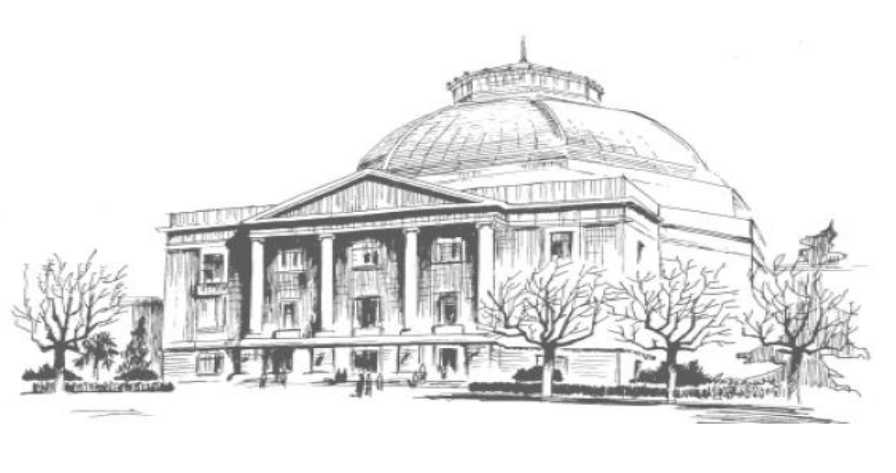
\includegraphics[width=0.9\textwidth]{pics/cover.png} \\[2pt]
        \textsc{\Huge Principles of Databases}\\[10pt]
        \begin{tabular}[c]{rc}
            Title       & \blankToFill{\thetitle} \\
            Date        & \blankToFill{\today} \\
            Author      & \blankToFill{\theauthor\footnotemark} \\
            Student ID  & \blankToFill{\thestudentID} \\
            Institution & \blankToFill{\theinstitution}
        \end{tabular}
        \rmfamily
    \end{center}
    \footnotetext{\theemail}
\end{titlepage}}

\newcommand{\result}[1]{

    The result see figure \ref{fig:query-#1}, and the complete code see list \ref{lst:query-#1}.

}

\newcommand{\src}[1]{
    
    \begin{listing}[hp]
        \centering
        \inputminted[bgcolor=codebg,autogobble,linenos=true,breaklines]{sql}{src/query#1.sql}
        \caption{Code of Query #1}
        \label{lst:query-#1}
    \end{listing}

}

\newcommand{\pic}[1]{
    
    \begin{figure}[hp]
        \centering
        \includegraphics[width=\textwidth]{pics/query#1.png}
        \caption{Result of Query #1}
        \label{fig:query-#1}
    \end{figure}

}

\begin{document}
    \makecover

    \tableofcontents

    \newpage

    \section{Assignment Requirements}

    \begin{itemize}
        \item Familiar with the powerful SQL query statements;
        \item Familiar with the cute Microsoft Windows 11.
    \end{itemize}

    \section{Platforms and Tools}

    \begin{itemize}
        \item Windows 11 22H2 22621.521;
        \item Microsoft Access for Microsoft 365 (2209 Build 16.0.15629.20152 64-Bit).
    \end{itemize}

    \section{Implementation Plan}

    \subsection{Create Database and Import Data}

    Skipping the operations of this section. For result of the import, see the attachment \verb|university.accdb|.

    \subsection{Answer the Questions}

    \subsubsection{Query 1}

    An easy task. Use \mintinline{sql}{WHERE P.dname = D.dname AND D.numphds < 50} to filter the records.

    \result{1}

    \subsubsection{Query 2}

    Select the lowest \verb|gpa| from table \verb|student|, then select the \verb|name| of \verb|student|(s) whose \verb|gpa| equals to it.

    \result{2}

    \subsubsection{Query 3}

    Join the \verb|student| table with \verb|enroll| table, then select the average \verb|gpa|, with grouping by \verb|cno| and \verb|sectno|.

    \result{3}

    \subsubsection{Query 4}

    An easy task. The key point of this task is to use the \verb|HAVING| clause to filter results.

    \textbf{Note that the maximum number of students is increased to 9, since we can select nothing when it was set to 6.}

    \result{4}

    \subsubsection{Query 5}

    Calculate how many courses each student has chosen, then find its maximum value, select the students that chose the same number of courses as the maximum.

    \result{5}

    \subsubsection{Query 6}

    Select the students that under 18 years old, then select their major departments.

    \result{6}

    \subsubsection{Query 7}

    Select the students that take one of the College Geometry courses, then select their names and majors.

    \result{7}

    \subsubsection{Query 8}

    Select the students that enrolled the class ``College Geometry*'', then select their majors. Finally select the departments that have no ``selected'' majors.

    \result{8}

    \subsubsection{Query 9}

    Select the students enrolled courses from ``Computer Sciences'', then select the students enrolled courses from ``Mathematics'' and selected before. Finally select their names.

    \result{9}

    \subsubsection{Query 10}

    Select all the students majored in ``Computer Sciences'', then calculate the minimum age and the maximum age, get their difference.

    \result{10}

    \subsubsection{Query 11}

    Group students by their majors, calculating all the averages. Then select the departments that have majors with gpa under 1.0.

    \result{11}

    \subsubsection{Query 12}

    Count the students' enrolls of ``Civil Engineering'', then select those whose count is equal to the count of courses that ``Civil Engineering'' has.

    \result{12}

    \section{Experimental Feelings}

    There are so much things \textit{Microsoft Access} does not support\dots I had nothing to say.

    \section{Codes}

    Here are all the codes written in the project.

    \listoflistings

    \src{1}
    \src{2}
    \src{3}
    \src{4}
    \src{5}
    \src{6}
    \src{7}
    \src{8}
    \src{9}
    \src{10}
    \src{11}
    \src{12}

    \clearpage
    
    \section{Results}

    Here are all the screenshots of results of the project's queries.

    \listoffigures

    \pic{1}
    \pic{2}
    \pic{3}
    \pic{4}
    \pic{5}
    \pic{6}
    \pic{7}
    \pic{8}
    \pic{9}
    \pic{10}
    \pic{11}
    \pic{12}
\end{document}